% ET722A Luciano Albuquerque Lima Saraiva
\documentclass[12pt,a4paper]{article}
\usepackage[utf8]{inputenc}
\usepackage[onehalfspacing]{setspace}
\usepackage[lmargin=3cm,tmargin=3cm,rmargin=2cm,bmargin=2cm]{geometry}
\usepackage[brazil]{babel}
\usepackage[T1]{fontenc}
\usepackage{graphicx}
\usepackage{indentfirst}
\usepackage{comment}
\usepackage{enumerate}
\usepackage{hyperref}
\usepackage{tabularx}
\usepackage{subfig}
\usepackage{glossaries}


\hypersetup{
    colorlinks=true,
    linkcolor=blue,
    filecolor=magenta,
    urlcolor=cyan,
}

% numeracao header
\pagestyle{headings}

% quebra de pagina por secao
\let\oldsection\section
\renewcommand\section{\clearpage\oldsection}

% glossário
\newglossaryentry{microcontroladora} {
	name = Microcontroladora,
	description = {
		Microcontrolador é um pequeno computador (SoC) num único circuito integrado
		o qual contém um núcleo de processador, memória e periféricos programáveis 
		de entrada e saída
	}
}
\newglossaryentry{ultras} {
	name=Ultrasônico,
	description = {
		Sinais Ultrassônicos são ondas mecânicas com frequência acima de 40 KHz
	}
}
\newglossaryentry{ulong} {
	name=ulong,
  description = {
		Tipo de dado para armazenamento de valores inteiros sem sinais longos,
		dependende do hardware no nosso caso armazena um total de 32 bits
	}
}

\newglossaryentry{bool} {
	name=bool,
	description = {
			Tipo de dado booleano 0 ou 1
	}
}

\newglossaryentry{uint8} {
	name=uint8,
	description = {
		Tipo de dados para armazenar valores inteiros sem sinais que variam até 8
		bits (255)
 }
}

\newglossaryentry{alfa} {
	name=alfa,
	description = {
		Caracteres alfas da tabela ASCII, A-Za-z
	}
}

\newglossaryentry{OLED} {
	name=OLED,
	description = {
		Diodo orgânico emissor de luz
	}
}

\makeglossaries

% bibliografia
\usepackage[nottoc,notlot,notlof]{tocbibind}


\begin{document}

\begin{titlepage}
	\begin{center}
		\textbf{UNIVERSIDADE DE RIBEIRÃO PRETO} \\
			CIÊNCIAS EXATAS \\
			Engenharia de Software I

			\vspace{1.5cm}

			\textbf{Prof. Luciano A. L. Saraiva}
			\vspace{0.5cm}

			\textbf{Murilo da Silva Ijanc'} \\
			RA: 834125

			\vspace{6.5cm}

			\textbf{DOCUMENTO DE REQUISITOS} \\
			\textbf{PIPI PET}

			\vfill

			\vspace{0.8cm}

			
\includegraphics[width=0.2\textwidth]{unaerp}

			\textbf{RIBEIRÃO PRETO} \\
			\textbf{2020}
	\end{center}
\end{titlepage}


\thispagestyle{empty}

\tableofcontents

\newpage

\thispagestyle{empty}
\listoftables
\thispagestyle{empty}
\listoffigures
\thispagestyle{empty}
\printglossary[type=main,style=long,nonumberlist]

\pagenumbering{arabic}

% secao 1
\section{Introdução}
Este documento especifica os requisitos necessários para o desenvolvimento do
sensor \textbf{Pipi Pet}.

O documento visa estabelecer um entendimento comum entre os envolvidos no
projeto a respeito das funcionalidades a serem contempladas pelo sensor, bem
como facilitar os testes e homologação do mesmo.

\subsection{Cliente}
Ana Luisa Trevizolli Esteves, universitária, 27 anos, mora em um apartamento
com seus dois pets.

\subsection{Problema}
Em ambientes pequenos como apartamentos os pets realizam suas necessidades
diárias próximo aos seus donos, exigindo uma maior atenção para manter o
ambiente higienizado e com cheio agradável. Qualquer demora na higienização
pode acarretar problemas irreversíveis para o ambiente, bem como para o pet
e seus donos.

\subsection{Descrição geral do sistema}
O sensor proposto oferece uma solução para identificar se o pet nas categorias
cão e gato realizou suas necessidades. A idéia central é promover um ambiente
mais higiênico para locais de pequeno porte como apartamentos e canis.

\subsection{Restrições do projeto}
\begin{itemize}
	\item O software do sensor necessariamente precisa ser desenvolvido na
		linguagem C/C++ e possua portabilidade para funcionar em
		\gls{microcontroladora}
	\href{http://ww1.microchip.com/downloads/en/DeviceDoc/doc7799.pdf}{ATMEGA16U2};
	\item O software deve ser entregue em um prazo máximo de 12 meses;
	\item O software deverá ser construído em paralelo com hardware;
	\item O projeto do software do sensor não pode ultrapassar R\$ 3.500,00;
\end{itemize}

\subsection{Descrição do método levantamento de requisitos}
Para o levantamento de requisitos foi realizado uma entrevista estruturada, ou
seja, foi elaborado uma lista de perguntas para extrair do cliente as
respectivas funcionalidades que o software deve possuir. Algumas perguntas
estão relacionadas abaixo:

\textbf{Observação}: As perguntas não foram realizadas nessa ordem umas vez que
durante a entrevista procurou identificar alguns comportamentos do cliente, no
qual serviu de métrica para abordagem das perguntas.

\begin{itemize}
	\item Você possui pet?
	\item Qual a frequência que seu pet realiza necessidades?
	\item Você higieniza toda vez que o pet realiza as suas necessidades ou espera
		ao final do dia?
	\item Hoje você possui alguma forma de alerta quando seu pet realiza suas
		necessidades?
	\item Sabe qual é área do seu apartamento?
	\item O seu pet faz as necessidade em um único ambiente do apartamento?
\end{itemize}

% secao 2
\section{Descrição da informação}

\subsection{Dicionário de Dados}

% Nome do atributo Chave Primaria Descrição Tipo de dado Tamanho
% Formatação/Mascara Domínio Obrigatório

\begin{table}[h!]
	\begin{tabularx}{\textwidth}{|l|X|l|X|l|X|l|X|l|l|l|l|}
	\hline
	Atributo & Ch. Prim. & Descrição & T. Dado & Tam. & Másc. & Dom. & Reque.\\
	\hline
		Código & S & Código do sensor & \gls{ulong} & $2^{32} - 1$ & N & 32 bits & S \\
		Status & N & Status do sensor & \gls{bool} & 1 & N & (V/S) & S \\
		Unidade & N & Unidade de medida & \gls{uint8} & $2^8 - 1$ & N & 8 bits & S \\
		Modelo & N & Modelo do sensor & \gls{alfa} & 4 & AAA & A-Z & S \\
	UltimoTempo & N & tempo de checagem & time & - & SS & - & S \\
		Versão & N & Versão do sensor & \gls{alfa} & 6 & MMP & 0-9 & S \\
	\hline
	\end{tabularx}
	\caption{Dicionário de dados}
	\label{table:1}
\end{table}

\subsection{Fluxograma}
\begin{figure}[htb!]
	\centering
	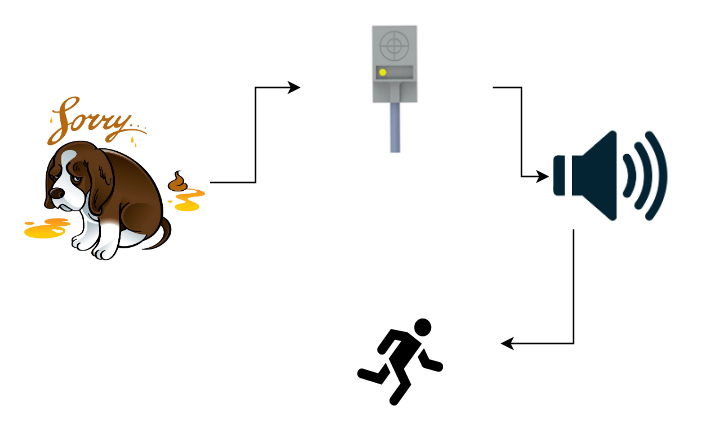
\includegraphics[width=13cm]{fluxograma}
	\caption{Fluxograma Sensor Pipi Pet}
	\label{fig:fluxograma}
\end{figure}

% secao 3
\section{Descrição da interface do sistema}

\subsection{Interface com o usuário}
A interface do usuário se faz através de um sensor de Oled I2C com
\gls{microcontroladora} SSD1306 que suporta 128x64 resolução em pixels.
\begin{figure}[htb!]
	\centering
	\subfloat[Boas vindas]{{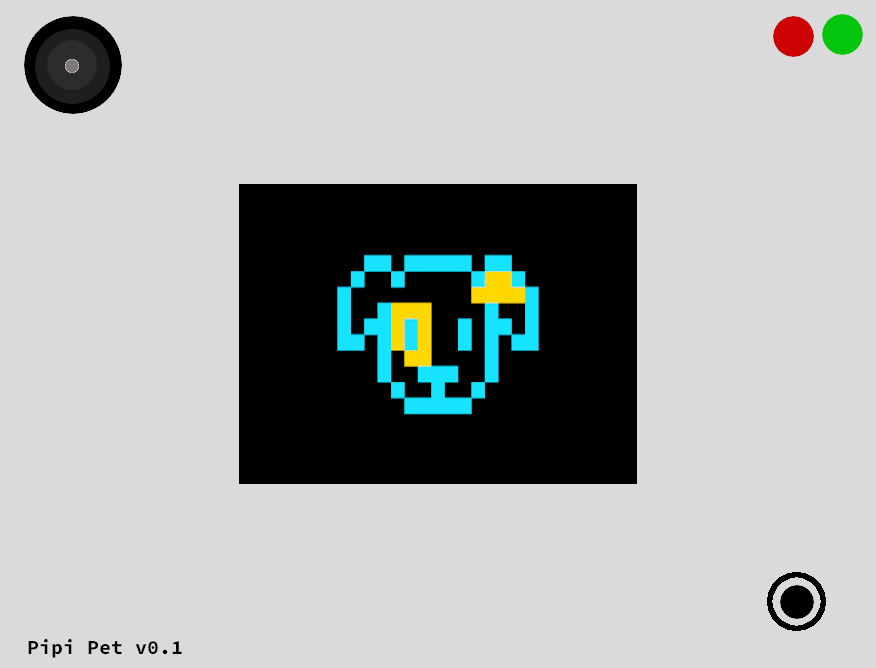
\includegraphics[width=6cm]{interface_1} }}
	\qquad
	\subfloat[Contagem de necessidades]
		{{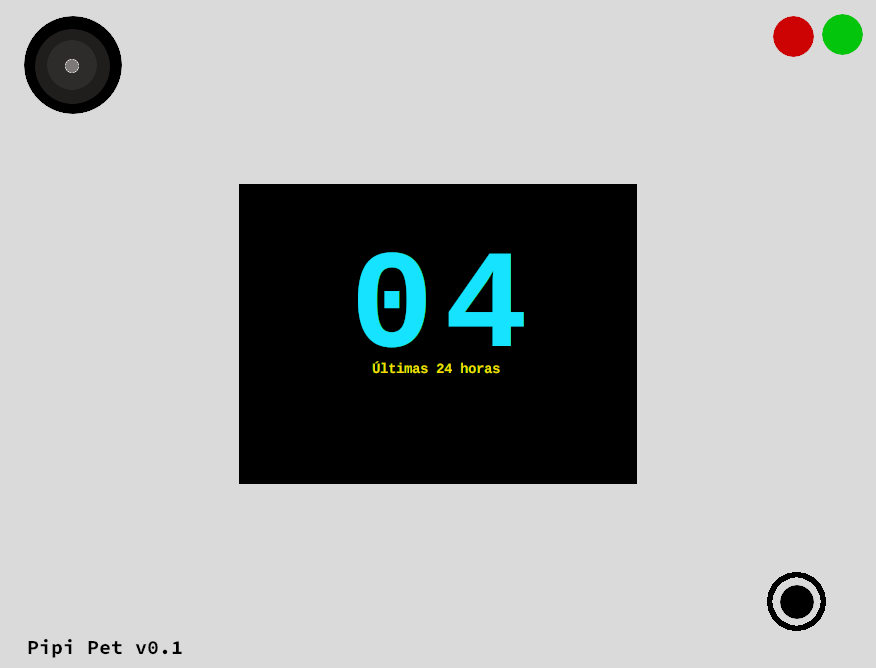
\includegraphics[width=6cm]{interface_2} }}
	\caption{Inteface Pipi Pet}
	\label{fig:interface}
\end{figure}

\subsection{Interface de comunicação}
A interface de comunicação é realizada através de uma porta serial, na qual
será possível coletar dados como:
\begin{itemize}
	\item registros de necessidades das últimas 24 horas;
	\item checar calibração do sensor;
\end{itemize}

% secao 4
\section{Descrições funcionais}

\subsection{Requisitos funcionais}
Nos requisitos funcionais são apresentadas as tarefas que o software necessita
realizar para atender as necessidades da solução.

\subsubsection{[RF001] Sincronizar relógio}
O sensor deve sincronizar a hora toda vez que cair a energia ou for
desligado.

\subsubsection{[RF002] Converter medida}
O sensor deve converter a medida para centimêtros para ficar fácil o
processo de medição por parte do usuário.

\subsubsection{[RF003] Emitir alerta sonoro}
O sensor deve emitir um alerta sonoro quando houver necessidades do pet.

\subsubsection{[RF004] Parar alerta sonoro}
O sensor deve parar o alerta após 3 tentativas de 30 segundos ou quando
pressionado o botão para parar pelo usuário.

\subsubsection{[RF005] Relatório visor}
O sensor deve emitir um relatório diário de quantas necessidades o pet
realizou nas últimas 24 horas.

\subsubsection{[RF006] Registrar necessidade do pet}
O sensor necessita registrar a data e a hora em que o pet realizou suas
necessidades.

\subsubsection{[RF007] Apagar necessidades do pet}
O sensor deve apagar as necessidades que são anteriores as últimas 24 horas.

\subsubsection{[RF008] Ascender o led}
O sensor deve ascender um led para indicar o status atual do sensor (ligado ou
desligado).

\subsection{Requisitos não funcionais}

\subsubsection{[NF001] Velocidade do sensor}
O sensor não pode atrasar mais do que 1 (um) segundo para ler os dados.

\subsubsection{[NF002] Uso software livre}
Para agilidade do processo de desenvolvimento os desenvolvedores devem utilizar
softwares de código aberto e de licença livre.

\subsubsection{[NF003] Tecnologias}
Para testar o código seria fundamental ter um simulador ou uma
\gls{microcontroladora} compátivel com a que será usada no projeto, como por exemplo
Arduino Uno, ESP32 ou ESP8266.

\subsubsection{[NF004] Controle de Versão}
Para equipe conseguir interagir entre as diferentes versões do software um
gerenciador de controle de versão é fundamental. No caso como o projeto pensa
em utilizar partes de software livre durante o desenvolvimento, seria
importante adotar uma solução não comercial para o controle de versão como por
exemplo: GIT, SVN, Mercurial ou CVS.

\subsubsection{[NF005] Integração Contínua}
Na liberação de novas releases é fundamental que tenha um processo de
integração para análisas de possíveis erros, dificultando problemas que possam
atrasar na liberação do software.

\subsection{Requisitos de produto e processo}
\subsubsection{Produto}
É fundamental que o software possa checar a disponibilidade dos sensores que
envolvam a solução. Abaixo os 3 sensores essenciais:
\begin{itemize}
	\item \gls{ultras}
		(\href{https://cdn.sparkfun.com/datasheets/Sensors/Proximity/HCSR04.pdf}{HCSR04})
	\item \gls{OLED}
		(\href{https://cdn-shop.adafruit.com/datasheets/SSD1306.pdf}{SSD1306})
	\item Sonoro
\end{itemize}

\subsubsection{Processo}
Como o projeto necessita de um hardware para solucionar o problema de
higienização das necessidades do pet, uma linguagem que atenda requisitos
por exemplo integrar com SDK da \gls{microcontroladora} e ao mesmo tempo possa ser
acessível para manipulação de memória, bits se faz necessário, por tanto uma
das linguagens que atende esses quesito é C/C++ podendo no futuro com mais
recursos do time usar Rust.

\subsection{Requisitos quantificáveis}
O sensor deve manter seu funcionamento 24 horas por dia 7 dias por semana com 
exceção dos momentos que não existir de forma alguma uma uma fonte de energia 
para o mesmo.

% secao 5
\bibliographystyle{ieeetr}
\bibliography{biblio}
\nocite{sommerville1997requirements}
\nocite{pressman2005software}
\nocite{project2000guide}
\nocite{de2003engenharia}
\nocite{wiki:Requisito_funcional}
\nocite{wiki:Sistema_de_controle_de_versoes}
\nocite{wiki:Continuous_integration}

\end{document}
